% ********** BEGIN Chapter 3 **********
\chapter{Background Study}
\label{sec:BackgroundStudy}

\section{VoIP Market}
\label{sec:BackgroundStudy:VoIPMarket}

In the telecom market, VoIP technology has gained more and more customers. The advantage of VoIP is obviously, much cheaper fee and almost same quality as traditional telephone.  Report from Infonetics indicates that, in the year 2007, the subscribers for VoIP are under 80 all around world. Most of them are in the Asia Pacific region. However by the year of 2011 the user will be 135 million, predicted by \textsf{MarketResearch.com}. And a UK research company \textsf{Disruptive Analysis Ltd.} predicts the users of mobile-VoIP will be 250 million by the year of 2012.\cite{StateOfTheVoIPMarket2008}

The analyses and figures above draw a brilliant future of VoIP market.  

\subsection{VoIP Service Provider}
\label{sec:BackgroundStudy:VoIPMarket:VoIPServiceProvider}

VoIP service provider is the company which supplies the products of VoIP/PSTN gateway. Or the ones who supply the service that customers can call a PSTN phone by a VoIP phone via their service/network. There are hundreds of such companies in the world. PSTN\label{sym:PSTN} is short for Public Switched Telephone Network. It is the network of the world's public circuit-switched telephone networks. In another word, it is just the traditional phone network.


\subsection{VoIP Client}
\label{sec:BackgroundStudy:VoIPMarket:VoIPClient}



\subsection{Solution Provider}
\label{sec:BackgroundStudy:VoIPMarket:SolutionProvider}



\section{Third Party Call Control}
\label{sec:BackgroundStudy:ThirdPartyCallControl}

In the traditional telephony context, third party call control allows one entity (which we call the controller) to set up and manage a communications relationship between two or ore other parties.  Third party call control (referred to as \textbf{3pcc}\label{sym:3pcc}) is often used for operator services (where an operator creates a call that connects two participants together) and conferencing.\cite{RFC3725}

\begin{figure}[!hbtp]
\centering
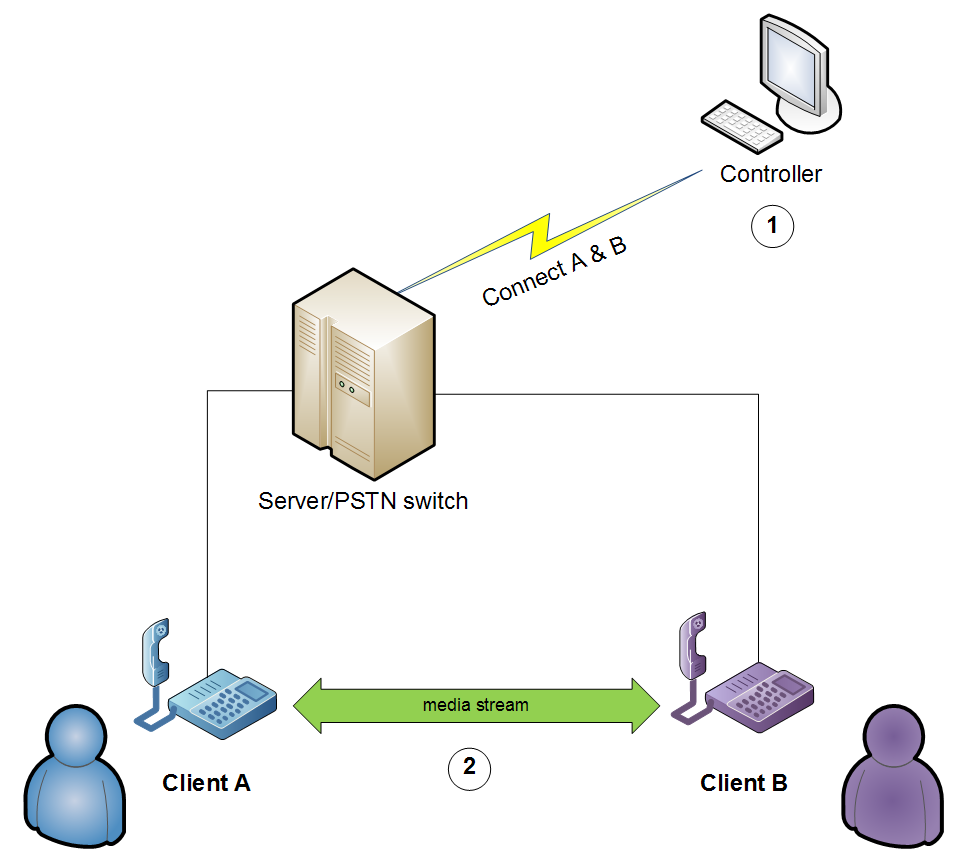
\epsfig{file=chap03/resources/3pcc, width=4in}
\caption{Third party call control}
\label{fig:ThirdPartyCallControl}
\end{figure}


A general work flow of 3pcc is shown in Figure \ref{fig:ThirdPartyCallControl}. The initial side of the phone is the \textit{controller}. The \textit{controller} sends a signal ``connect \textit{client \nolinebreak A} and \textit{client \nolinebreak B}'' to the server \hyperref[fig:ThirdPartyCallControl]{\ding{172}}. And the server establishes a call between \textit{client A} and \textit{B} \hyperref[fig:ThirdPartyCallControl]{\ding{173}}.

\section{3pcc in VoIP}
\label{sec:BackgroundStudy:3pccInVoIP}


% ********** End of chapter 3 **********
